\documentclass{article}

\usepackage{amsmath}
\usepackage{graphicx}

\title{Title of my document}
\date{2013-09-01}
\author{John Doe}



\begin{document}

\maketitle

\pagenumbering{gobble}

\newpage

\pagenumbering{arabic}

\section{Section}

Hello World!

\subsection{Subsection}

Structuring a document is easy!

\subsubsection{Subsubsection}

More text.

\paragraph{Paragraph}

Some more text.

\subparagraph{Subparagraph}

Even more text. This formula $f(x) = x^2$ is an example.

\section{Another section}
Fig \ref{figure:boat1} shows a boat.


\begin{equation*}
  1 + 2 = 3
\end{equation*}

\begin{equation*}
  1 = 3 - 2
\end{equation*}

\begin{align*}
  1 + 2 &= 3\\
  1 &= 3 - 2
\end{align*}

\begin{align*}
  f(x) &= x^2\\
  g(x) &= \frac{1}{x}\\
  F(x) &= \int^a_b \frac{1}{3}x^3\\
  \frac{1}{\sqrt{x}}
\end{align*}

\begin{equation*}
  \left[
  \begin{matrix}
  1 & 0\\
  0 & 1
  \end{matrix}
  \right]
\end{equation*}

\begin{equation}
  f(x) = x^2
\end{equation}

\begin{figure}[h!]
  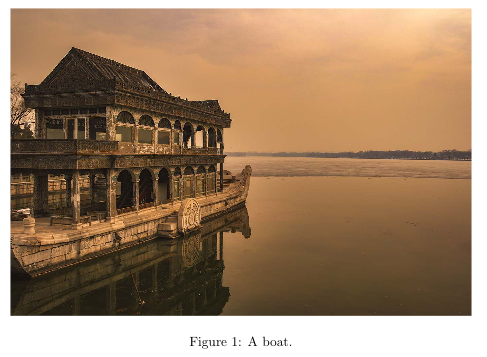
\includegraphics[width=\linewidth]{boat.png}
  \caption{A boat}
  \label{figure:boat1}
\end{figure}

This is some example text\footnote{\label{myfootnote}Hello footnote}.


I'm referring to footnote \ref{myfootnote}.

\end{document}
